% TODO
% Add footnotes
% Print this pdf

\documentclass [12pt, letterpaper, twoside] {article}
\usepackage[utf8]{inputenc}
\usepackage [left=1.0in, right=1.0in, top=1.0in, bottom=1.0in] {geometry}
\usepackage {datetime}
\usepackage {tikz}
\usepackage {caption}
\usepackage {amsmath}
\usepackage {tabu}
\usepackage {multirow}
\usepackage {verbatim}
\usepackage {caption}
\usepackage {float}
\usepackage {cancel}
\usepackage {pgfplots}

\usetikzlibrary {shapes.geometric, arrows}

\tikzstyle {pink1circle0} = [circle, minimum size=0.5cm, text centered, draw=black, fill=pink1]
\tikzstyle {arrow} = [thick, ->, >=stealth]
\renewcommand {\labelitemiv}{$\triangle$}

\raggedbottom
\begin {document}
\begin {titlepage}
\begin {center}
Department of Biological, Chemical, and Physical Science\\
\vspace {0.1cm}
Illinois Institute of Technology\\
\vspace {0.1cm}
General Physics I: Mechanics (PHYS 123-02)\\
\vspace* {\fill}
\begingroup
\Large
\textbf {Newton's 2nd Law}
\vspace {0.35cm}

\normalsize
Lab 3
\vspace {1.5cm}
\endgroup
\vspace* {\fill}
\end {center}

\vspace*{\fill}
\begin {flushright}
\footnotesize
Emily Pang, Coby Schencker (lab partner)\\
Date of experiment: 12 Sept 2019\\
Due date: 19 Sept 2019\\
Lab section L04\\
TA: Mithila Mangedarage\\
Updated \usdate\today~(\currenttime)
\end {flushright}
\end {titlepage}
\pgfplotsset{compat=1.7}
\subsection* {STATEMENT OF OBJECTIVE}
The objective of this lab was to devise and conduct experiments that tested Newton's 2nd Law and proved that it is impossible to use a simple inclined plane to test whether acceleration was inversely proportional to the mass

\subsection* {THEORY}
\noindent
The basis of these experiments rest on determining whether Newton was correct in his 2nd Law of Motion:
\begin {equation}
  \begin {split}
    \vec{F}_{\text{net}} = m\vec{a} \\
  \end {split}
\end {equation}
with units Newtons. When the system we are investigating is on a simple inclined plane, then it becomes important to define the \(xy\) plane. For our experiment, we declared the \(x\) direction as parallel to the hypotenuse of the incline plane and the \(y\) direction as perpendicular to the hypotenuse.Thus, we have the following equation for the forces in the \(x\) direction:
\begin {equation}
  \begin {split}
    F_{g}\sin{\theta} & = m\vec{a} \\
    \cancel{m}{}g\sin{\theta} & = \cancel{m}{}a \\
    g\sin{\theta} & = a \\
  \end {split}
\end {equation}
\(\theta\) can be found by measuring either the angle or the two sides. To verify the acceleration from Newton's 2nd Law, we used a kinematics equation and solved for \(a\) as follows
\begin {equation}
  \begin {split}
    v_{f}^2 & = \cancelto{0}{v_{0}^2}+2a\Delta{x} \\
    a & = \dfrac{v_{f}^2}{2\Delta{x}} \\
  \end {split}
\end {equation}
As shown we start the experiment with an intial velocity of zero. In this equation, we can control \(\Delta{x}\) and measure \(v_{f}\). The resulting equations combined is as follows
\begin {equation}
  \begin {split}
     g\sin{\theta} & = \dfrac{v_{f}^2}{2\Delta{x}} \\
  \end {split}
\end {equation}
Note that the mass cancels out in these equations, showing that mass cannot be shown to be proportional using a simple inclined plane. However, the devised experiment outlined in the procedure below will show it explicitly. For the first experiment, in order to prove whether Newton's 2nd Law was correct in acceleration being proportional to the effective force applied to the glider, we will measure \(\theta\), \(v_{f}\), and \(\Delta{x}\). If both sides are equal, then we show that Newton's 2nd Law holds for the aforementioned proportionality. 

\subsection* {EQUIPMENT}
  \noindent
  \begin {itemize}
    \itemsep0em
    \item {one PASCO Capstone software}
    \item {one glider}
    \item {one air track}
    \item {one dial caliper}
    \item {one scale}
    \item {one meter stick}
    \item {four 20 gram weights}
    \item {one photogate}
    \item {four wooden blocks}
    \item {one white flag}
  \end {itemize}

\subsection* {PROCEDURE}
For the first experiment, we first recorded \(\Delta{x}\), or from where the glider started to when it was recorded by the photogate. We then recorded three different masses of the glider: the glider itself and the glider with varying amounts of supplemental masses. Each time \(\theta\) was changed, the distance the air track was lifted and the distance from the wooden blocks to the end of the air track was recorded as well, as we didn't have a protractor. Finally, for each variation in \(\theta\), the average velocity calculated by the photogate was recorded by measuring the time the white flag took to pass the photogate. \\\\
Note that since the mass was varied with each new \(\theta\), we can verify whether the mass changes the acceleration and matches what our theoretical findings showed us in Equation Set 2.

\subsection* {DATA}
The data is as follows for the experiments:
\begin {table}[h]
  \centering
  \begin {tabular}{| l | r | r | r |}
    \hline\hline
    & Opposite (m) & Adjacent (m) & Resulting \(\theta\) \\
    \hline
    Angle 1 & 0.00790 & 1.370 & 0.330 \\ %388059
    \hline
    Angle 2 & 0.0344 & 1.330 & 1.48 \\ %1605622
    \hline
    Angle 3 & 0.0580 & 1.220 & 2.72 \\ %1848358
    \hline
    Angle 4 & 0.0842 & 1.295 & 3.72 \\ %0095414
    \hline\hline
  \end {tabular}
  \caption {Calculated Angles}
\end {table}

\begin {table}[h]
  \centering
  \begin {tabular}{| l | r | r | r |}
    \hline\hline
    & \(m_{1}\) & \(m_{2}\) & \(m_{3}\) \\
    \hline
    & 0.1968 & 0.2367 & 0.2769 \\
    Measured Mass (kg) & 0.1967 & 0.2367 & 0.2769 \\
    & 0.1967 & 0.2367 & 0.2768 \\
    \hline
    Avg. Mass (kg) & 0.1967 & 0.2367 & 0.2769 \\ %33333 % %66667 (last digit rounded)
    \hline\hline
  \end {tabular}
  \caption {Average Masses}
\end {table}

\begin {table}[h]
  \centering
  \begin {tabular}{| l | r | r | r | r |}
    \hline\hline
    & \(v_{f}\) of \(m_{1}\) (\(\tfrac{\text{m}}{\text{s}}\)) & \(v_{f}\) of \(m_{2}\) (\(\tfrac{\text{m}}{\text{s}}\)) & \(v_{f}\) of \(m_{3}\) (\(\tfrac{\text{m}}{\text{s}}\)) & Avg Velocity (\(\tfrac{\text{m}}{\text{s}}\)) \\
    \hline
    \multirow {3}{*}{\(\theta=0.330\)} & 0.24 & 0.20 & 0.20 & \\
    & 0.20 & 0.19 & 0.20 & \\
    & 0.24 & 0.20 & 0.20 & \\
    \hline
    Avg \(v_{f}\) (\(\tfrac{\text{m}}{\text{s}}\)) & 0.23 & 0.20 & 0.20 & 0.21 \\ %6666667 (LDR) %666667 (LDR) % %7777779 (LDR)
    \hline
    \multirow {3}{*}{\(\theta=1.48\)} & 0.48 & 0.45 & 0.45 & \\
    & 0.47 & 0.45 & 0.45 & \\
    & 0.48 & 0.45 & 0.45 & \\
    \hline
    Avg \(v_{f}\) (\(\tfrac{\text{m}}{\text{s}}\)) & 0.48 & 0.45 & 0.45 & 0.46 \\ %6666667 (LDR) % % %8888889 (LDR)
    \hline
    \multirow {3}{*}{\(\theta=2.72\)} & 0.61 & 0.61 & 0.61 & \\
    & 0.62 & 0.61 & 0.61 & \\
    & 0.61 & 0.61 & 0.61 & \\
    \hline
    Avg \(v_{f}\) (\(\tfrac{\text{m}}{\text{s}}\)) & 0.61 & 0.61 & 0.61 & 0.61 \\ %3333333 % % %1111111
    \hline
    \multirow {3}{*}{\(\theta=3.72\)} & 0.74 & 0.74 & 0.74 & \\
    & 0.74 & 0.74 & 0.74 & \\
    & 0.74 & 0.74 & 0.74 & \\
    \hline
    Avg \(v_{f}\) (\(\tfrac{\text{m}}{\text{s}}\)) & 0.74 & 0.74 & 0.74 & 0.74 \\
    \hline\hline
  \end {tabular}
  \caption {Velocities for varying angles and masses}
\end {table}
\begin {comment}
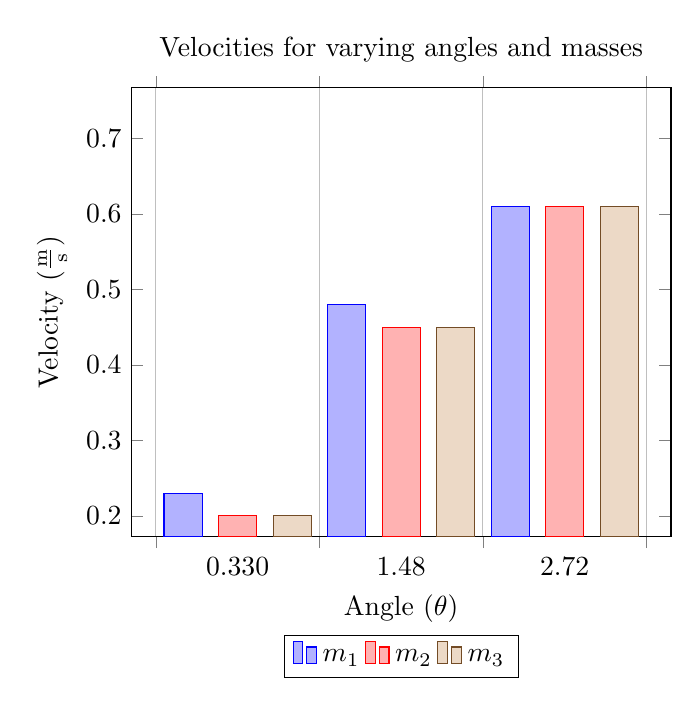
\begin{tikzpicture}
\begin{axis}[
    title = {Velocities for varying angles and masses},
    ybar,
    ybar interval = 0.7,
    enlargelimits=0.05,
    legend style={at={(0.5,-0.22)},
      anchor=north,legend columns=-1},
    xlabel={Angle (\(\theta\))},
    ylabel={Velocity (\(\tfrac{\text{m}}{\text{s}}\))},
    symbolic x coords={0.330,1.48,2.72,3.72},
    xtick=data,
    bar width = 5pt,
    %nodes near coords,
    %nodes near coords align={vertical},
    ]
\addplot coordinates {(0.330,0.23) (1.48,0.48) (2.72,0.61) (3.72,0.74)};
\addplot coordinates {(0.330,0.20) (1.48,0.45) (2.72,0.61) (3.72,0.74)};
\addplot coordinates {(0.330,0.20) (1.48,0.45) (2.72,0.61) (3.72,0.74)};

\legend {\(m_{1}\),\(m_{2}\),\(m_{3}\)}
\end{axis}
\end{tikzpicture}
\end {comment}

\begin {figure}[h]
\centering
  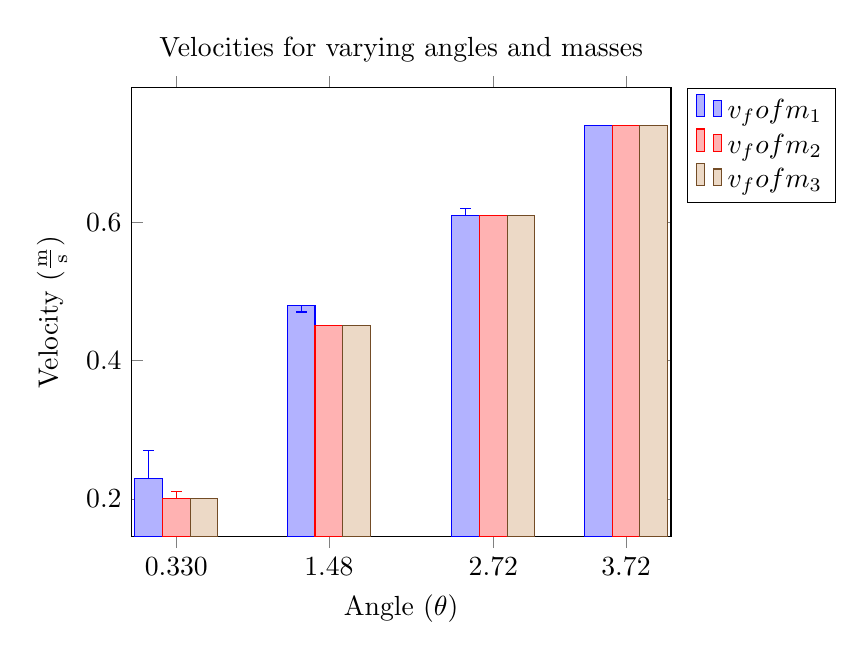
\begin{tikzpicture}
    \begin{axis}[
    legend pos=outer north east,
    %enlargelimits={abs=0.5},
    ybar=0pt,
    title = {Velocities for varying angles and masses},
    %bar width=0.15,
    %xtick={0.5,1.5,...,5.5},
    xticklabels={0.330,1.48,2.72,3.72},
    %symbolic x coords={0.330,1.48,2.72,3.72},
    xlabel={Angle (\(\theta\))},
    ylabel = {Velocity (\(\tfrac{\text{m}}{\text{s}}\))},
    %x tick label as interval
    xtick=data,
    ]

    \addplot+[error bars/.cd,
    y dir=plus,y explicit]
    coordinates {
      (0.330,0.23) +- (0.0, 0.04)
      (1.48,0.48) +- (0.0, -0.01)
      (2.72,0.61) +- (0.0, 0.01)
      (3.72,0.74) +- (0.0, 0.0)};
    \addplot+[error bars/.cd,
    y dir=plus,y explicit]
    coordinates {
      (0.330,0.20) +- (0.0, 0.01)
      (1.48,0.45) +- (0.0, 0.0)
      (2.72,0.61) +- (0.0, 0.0)
      (3.72,0.74) +- (0.0, 0.0)};
    \addplot+[error bars/.cd,
    y dir=both,y explicit]
    coordinates {
      (0.330,0.20) +- (0.0, 0.0)
      (1.48,0.45) +- (0.0, 0.0)
      (2.72,0.61) +- (0.0, 0.0)
      (3.72,0.74) +- (0.0, 0.0)};
    \legend{\(v_{f} of m_{1}\),\(v_{f} of m_{2}\),\(v_{f} of m_{3}\)}
    \end{axis}
  \end{tikzpicture}
\end {figure}

The meter and dial caliper were used to measure the distances, while the photogate measured the final (average) velocity for each glider run. The scale was used to record the masses of each glider.

\subsection* {ANALYSIS OF DATA}
The two sides of Equation 4 are calculated in the table below. 
\begin {table}[h]
  \centering
  \begin {tabular}{| l | c | c | c | c | c |}
    \hline\hline
    Angle & Eq 2 Calc & Eq 2 Result & Eq 3 Calc & Eq 3 Result & PE (\%) \\
    \hline
    \(\theta=0.330\) & (9.8)\(\tfrac{\text{m}}{\text{s}}\sin(0.330)\) & 0.057 & \(\dfrac{(0.21\tfrac{\text{m}}{\text{s}})^2}{2(0.478)\text{m}}\) & 0.045 & 25 \\ %510009 (LDR) %7777779 %158583 %.1368073
    \hline
    \(\theta=1.48\) & (9.8)\(\tfrac{\text{m}}{\text{s}}\sin(1.48)\) & 0.25 & \(\dfrac{(0.46\tfrac{\text{m}}{\text{s}})^2}{2(0.478)\text{m}}\) & 0.22 & 15 \\ %3388942 %8888889 (LDR) %0270934 %.035124
    \hline
    \(\theta=2.72\) & (9.8)\(\tfrac{\text{m}}{\text{s}}\sin(2.72)\) & 0.47 & \(\dfrac{(0.61\tfrac{\text{m}}{\text{s}})^2}{2(0.478)\text{m}}\) & 0.39 & 19 \\ %5376027 %1111111 %0645178 %.1301092
    \hline
    \(\theta=3.72\) & (9.8)\(\tfrac{\text{m}}{\text{s}}\sin(3.72)\) & 0.64 & \(\dfrac{(0.74\tfrac{\text{m}}{\text{s}})^2}{2(0.478)\text{m}}\) & 0.57 & 11 \\ %5846583 %2803347 %.0060872
    \hline\hline
  \end {tabular}
  \caption {Calculated results from each side of Equation 4}
\end {table}
As shown in Table 3, the velocities for each of the angles did not vary much from mass to mass. When they did, it was extremely marginal. Data in this table also shows that the velocity increase when the angle increased. \\\\
Data in Table 4 shows the results from calculations done to both of the sides of Equation 4 given the data from the experiments. The PE, or percentage error, was calculated by dividing the subtraction of the two results by whichever result gave the larger percent error. The result was then multiplied by 100. \\\\
The graph below shows a visual representation of the velocities for each of the masses and their angles.

\subsection* {DISCUSSION OF RESULTS}
Since the aim of the first experiment was the test Newton's 2nd Law, we find that the results from both sides seem fairly close, confirming the relationship between the acceleration and the effective force applied to the glider. However, the PE's for the results are relatively high objectively, which could be due to measurement error most likely with measuring the sides of the incline plane. \\\\
For the second experiment, we showed that the mass did not have an effect on the acceleration, which makes sense with out earlier theoretical calculations. This is represented very clearly with the bar plot of the velocities.

\subsection* {FURTHER STUDY}
While the study confirmed our theoretical calculations, further study would serve as support for our conclusions. The points of weakness for our experiments include the position of the flag, which may have been altered on the glider throughout the experiment, and measuring the sides of the triangle formed from the air track, which were measured only once. Additionally, when measuring the sides of the triangle, we had to account for the bolts sticking out of the track, adding to another source of potential errors. Further experiments would be better off using a completely flat track to make measuring easier.

\subsection* {SUPPLEMENTAL QUESTIONS}
1. The calculated accelerations for Equations 2 and 4 (in the lab document) are shown in Table 4 under Equation 2 and Equation 3 respectively. \\\\
2. To derive an expression for normal force, we first look at Newton's 1st Law outlined in Equation 1. From there, we know that the only force acting on the glider is gravity, and by defining the \(y\) direction as perpendicular to the hypotenuse of the air track, we get
\begin {equation}
  \begin {split}
    F_{\text{N}}-F_{\text{g}}\cos(\theta) & = m\vec{a} \\
    F_{\text{N}}-\cancelto{}{m}g\cos(\theta) & = \cancelto{}{m}\vec{a} \\
    F_{\text{N}}-g\cos(\theta) & = \cancelto{0}{a} \\
    F_{\text{N}} & = g\cos(\theta) \\
  \end {split}
\end{equation}
where \(m\) is the mass of the glider, \(g\) is the acceleration of gravity and \(\theta\) is the angle of the inclined plane. Since the acceleration in our defined \(y\) direction is zero, then the forces, the normal force and gravity force, are equal. We can do a simply calculation using one of the angles to determine its normal force; in this case, we'll use \(\theta=2.72\).
\begin {equation}
  \begin {split}
    F_{\text{N}} & = g\cos(\theta) \\
    F_{\text{N}} & = (9.8\tfrac{\text{m}}{\text{s}}^2)\cos(2.72) \\
    F_{\text{N}} & = 9.8 \text{N} \\ %88944026 (LDR)
  \end {split}
\end {equation}

\noindent
If \(\theta\) is equal to 90, then we calculate the normal force as
\begin {equation}
  \begin {split}
    F_{\text{N}} & = g\cos(\theta) \\
    F_{\text{N}} & = (9.8\tfrac{\text{m}}{\text{s}}^2)\cos(90) \\
    F_{\text{N}} & = 0 \text{N} \\
  \end {split}
\end {equation}

\noindent
If \(\theta\) is zero, or the glider is on a horizontal surface, then the following equation shows the net forces in the \(y\) direction:
\begin {equation}
  \begin {split}
    F_{\text{net}} & = F_{\text{N}} - F_{\text{g}} = 0 \\
    F_{\text{N}} & = F_{\text{g}} \\
    F_{\text{N}} & = mg \\
  \end {split}
\end {equation}
Thus, when the air track is horizontal, the glider's normal force is equal to the force of gravity. \\

\noindent
3. If we were to push the glider up the frictionless incline with an inital velocity, then we could calculate the distance it would travel up the plane, using the conservation of energy:
\begin {equation}
  \begin {split}
    E_{i} & = E_{f} \\
    \cancelto{0}{PE_{i}}+KE_{i} & = PE_{f}+\cancelto{0}{KE_{f}} \\
    \dfrac{1}{2}\cancelto{}{m}v_{i}^2 & = \cancelto{}{m}gd\sin(\theta)\\
    \dfrac{1}{2}v_{i}^2 & = gd\sin(\theta) \\
    d & = \dfrac{v_{i}^2}{2g\sin(\theta)} \\
    d & = \dfrac{(0.61(\tfrac{\text{m}}{\text{s}}))^2}{2(9.8\tfrac{\text{m}}{\text{s}^2})\sin(2.72)} \\
    d & = 0.40\text{m} \\ %1241972
  \end {split}
\end {equation}
To find the time it would take for it to be launched and return to its starting position at \(\theta=2.72\), we use Newton's 1st Law (Equation 1).
\begin {equation}
  \begin {split}
    \vec{F}_{\text{net}} & = m\vec{a} \\
    \cancelto{}{m}g\sin(\theta) & = \cancelto{}{m}(\dfrac{\cancelto{0}{v_{f}}-v_{i}}{t}) \\
    g\sin(\theta) & = \dfrac{v_{i}}{t} \\
    t & = \dfrac{v_{i}}{g\sin(\theta)} \\
    t & = \dfrac{0.61(\tfrac{\text{m}}{\text{s}})}{(9.8\tfrac{\text{m}}{\text{s}^2})\sin(2.72)} \\
    t & = 1.3\text{s} \\ %13155545
  \end {split}
\end {equation}

\end {document}
